% This file was created by matlab2tikz.
%
%The latest updates can be retrieved from
%  http://www.mathworks.com/matlabcentral/fileexchange/22022-matlab2tikz-matlab2tikz
%where you can also make suggestions and rate matlab2tikz.
%
\documentclass[tikz]{standalone}
\usepackage[T1]{fontenc}
\usepackage[utf8]{inputenc}
\usepackage{pgfplots}
\usepackage{grffile}
\pgfplotsset{compat=newest}
\usetikzlibrary{plotmarks}
\usepgfplotslibrary{patchplots}
\usepackage{amsmath}
\usetikzlibrary{shapes.misc}

\usetikzlibrary{decorations.markings}

\tikzset{cross/.style={cross out, draw=black, ultra thick, minimum size=2*(#1-\pgflinewidth), inner sep=0pt, outer sep=0pt},
%default radius will be 1pt. 
cross/.default={1pt}}

\begin{document}
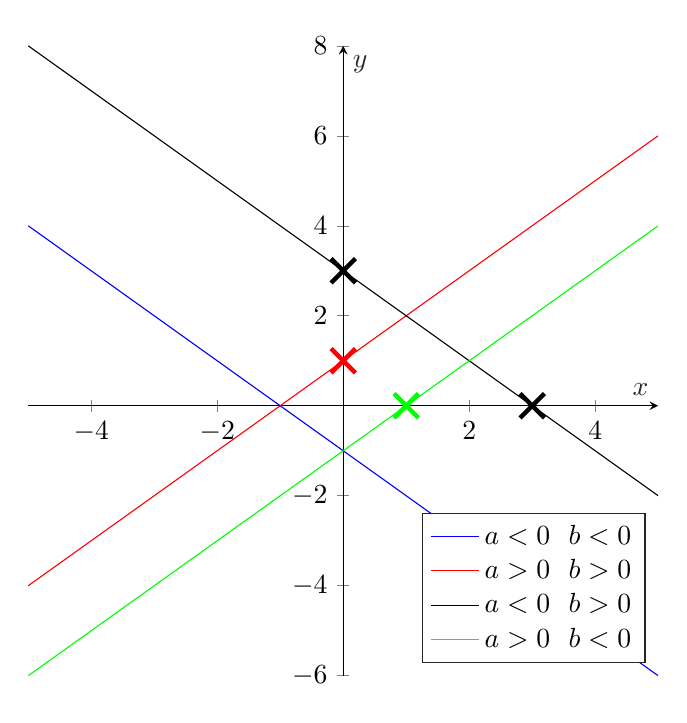
\begin{tikzpicture}

\begin{axis}[%
at={(0cm,0cm)},
axis lines=middle,
width=8cm,
height=8cm,
scale only axis,
xminorticks=true,
xlabel style={font=\color{white!15!black}},
xlabel={$x$},
yminorticks=true,
ylabel style={font=\color{white!15!black}},
ylabel={$y$},
axis background/.style={fill=white},
legend style={legend cell align=left, align=left, draw=white!15!black, at={(0.98,0.02)}, anchor=south east},
no markers
]

\addplot {-x - 1};
\addplot{x  + 1};
\addplot[color=black]{-x + 3};
\addplot[color=green]{x - 1};
\legend{$a < 0~~b<0$, $a > 0 ~~b>0$, $a < 0~~ b > 0$, $a > 0 ~~b<0$};
\draw (1,0) node[cross=6pt,green]{};
\draw (3,0) node[cross=6pt,black]{};
\draw (0,3) node[cross=6pt,black]{};
\draw (0,1) node[cross=6pt,red]{};

\end{axis}
\end{tikzpicture}%
\end{document}